\documentclass{school-22.101-notes}
\date{October 24, 2011}

\begin{document}
\maketitle

\lecture{Nucleon-Nucleon Scattering}
We have discussed the bound state of a deuteron (a neutron plus a proton) in Chapter~\ref{2H-bound-state}. To gain more insights for the essential properties of nuclear force, we will look at scattering of a neutron by a proton, in particular taking into account the l-s coupling in $V_{\mathrm{nuc}}$. 


For this chapter, we are going to use relations, 
\begin{itemize}
\item QM flux: 
  \eqn{ \vec{J} = \frac{i \hbar}{2 \mu} (\psi \gradient \psi^* - \psi^* \gradient \psi) }
  For instance, in spherical coordinate system, 
  \eqn{ \vec{J} &= \frac{\hbar}{2 i m} \left[ \psi^* \gradient \psi - \psi \gradient \psi^* \right] = \frac{\hbar}{2 \mu i} \left[ \psi^* \dpsidr - \psi \dpsidr^* \right] }
\item Mass conservation: 
  \eqn{ \ddt (\psi^* \psi) + \divergence \vec{J} = 0 }
\end{itemize}


Reference: Krane 4.2, 11.8., Liboff 14.1.






\topic{Scattering Cross Sections}
Recall that the scattering cross-section of neutron from proton is around 20 barns for $1 \sim 10^6$ eV \footnote{it is not till we introduce spin-spin coupling that we can explain this high scattering cross section}. 

To derive relations about the scattering cross section, we start by defining the incoming wave as a planar wave, and the outgoing wave as a spherical one. We define the scattering amplitude $f(\theta)$ as in $\psi_{\mathrm{sc}} = f(\theta) \frac{e^{i (\uline{k} \uline{r} - wt)}}{r}$. 
\begin{align}
\psi_{\mathrm{inc}} &= e^{i (\uline{k} \uline{r} - wt)} = e^{ikz}  = e^{ikr \cos \theta} 
&J_{\mathrm{inc}} &= \frac{\hbar k}{\mu} \\
\psi_{\mathrm{sc}} &=  f(\theta) \frac{e^{i (\uline{k} \uline{r} - wt)}}{r} = f(\theta) \frac{e^{ikr}}{r} &J_{\mathrm{sc}} &= \frac{\hbar k}{\mu r^2} |f(\theta)|^2 \\
\sigma(\theta) &= \mbox{Angular Differential xs} = \dsigmadOmega  &\sigma &= \int \sigma(\theta) \dOmega
\end{align}

Cross section is the probability that an incoming wave scatters along the solid angle $\Omega+\dOmega$. If we specify a small area on the spherical surface along the solid angle $\Omega$, then we can represent the area with $\Omega$:
\begin{align}
\dA &= r^2 \dOmega = r^2 \sin \theta \dtheta \dphi \\
\dsigma J_{\mathrm{inc}} &= J_{\mathrm{sc}} \dA = J_{\mathrm{sc}} r^2 \dOmega \\
\dsigmadOmega &= \frac{J_{\mathrm{sc}} r^2}{J_{\mathrm{inc}}} = \sigma(\theta) 
\end{align}

In the limit of $r \to \infty$ (we would prove this relation at the end), 
\eqn{ \psi &\approx e^{ikr \cos \theta} + f(\theta) \frac{e^{ikr}}{r} }
where $f(\theta)$ is the angular modulation, and the $\frac{e^{ikr}}{r}$ is the spherical wave. 
\eqn{ J_r &\approx \frac{|f(\theta)|^2}{r^2} \frac{\hbar k}{\mu}  & \Rightarrow r^2 \dOmega J_r &= |f(\theta)|^2 J_{in}}
We can derive the relation for differential scattering cross section $\dsigmadOmega$ and the total scattering cross section $\sigma$, 
\begin{align}
\left. \begin{array}{c}
J_{\mathrm{inc}} = \frac{\hbar k}{\mu} b^2  \\
J_{\mathrm{sc}} = \frac{\hbar k}{\mu r^2} b^2 |f(\theta)|^2 \\
\end{array} \right\} & \Rightarrow \boxed{\dsigmadOmega =  \frac{J_{\mathrm{sc}} r^2}{ J_{\mathrm{inc}}} = |f(\theta)|^2 }  \\
\Aboxed{ \sigma &= \int \dOmega |f(\theta)|^2  = 2 \pi \int_{\pi}^0 \derivative \cos \theta |f(\theta)|^2 }
\end{align}
Notes of scattering amplitude $f(\theta)$: 
\begin{enumerate}
\item $f(\theta)$ is scattering intensity as a function of scattering angle.
\item Generally $f(\theta)$ is anisotropic. For $l=0$ though there is no angular dependency, $f(\theta) \to $ constant. 
\item Angular differential xs $\sigma(\theta)$ is proportional to the scattering amplitude squared. Total scattering cross section is just angular differential cross section integrated over all angles.  
\item To solve for $f(\theta)$, use Method of Partial Waves. The result is in Eq.~\ref{f-theta}. 
\end{enumerate}


\topic{Born's Approach To Get Extreme Condition}
This lecture was given by Prof. Li on 10/22/12. We assume that the proton is stationary, the neutron is a travelling wave (thus we know the energy should be $\displaystyle E = \frac{\hbar^2 k^2}{2\mu}$, thus we can simplify the SQE (where $x$ is the relative location): 
\begin{align}
\left[ - \frac{\hbar^2 \nabla^2}{2 \mu} + V(|x|) \right] \psi(x) &= E \psi(x) \\
\left[ \nabla^2 - \frac{2 \mu V(|x|)}{\hbar^2} \right] \psi(x) &= - k^2 \psi(x) \\
(\nabla^2 + k^2) \psi(x) &= \frac{2 \mu V(|x|)}{\hbar^2} \psi(x) \label{scat-seq}
\end{align}
Mathamatically, we know the solution to $\displaystyle (\laplacian + k^2) G(x) = \delta(x)$ is the Green's function in the form of $\displaystyle G(x) = - \frac{e^{ik|x}}{4 \pi |x|}$. Notice, when $r$ is small, $G(x) \to - \frac{1}{4 \pi |x|}$. This is good because we can easily show that $\displaystyle \laplacian \left( - \frac{1}{4 \pi |x|} \right) = \delta (x)$. That is, 
\eqn{ (\laplacian + k^2) \psi(x) &= \delta(x - x') & \psi(x) &= - \frac{e^{ik |x - x'|}}{4 \pi |x-x'|} }
That is to say, the solution to Eq.~\ref{scat-seq} should be, 
\eqn{ \psi(x) &= e^{ikx} + \int \dV \frac{2 \mu V(|x'|) \psi(x')}{\hbar^2} \left( - \frac{e^{ik|x-x'|}}{4 \pi |x-x'|}  \right) }
The above equation we arrives at is the Born's approach. It is not a final solution because it requires us to have knowledge of $\psi(x')$ to solve for $\psi(x)$. But Born was able to show that this form is useful for $r\to \infty$ senario (because $x'$ is bound, then when $x$ becomes large, $x'$ can be ignored), 
\begin{align}
|x-x'| &= \sqrt{(x-x')(x-x')} = \sqrt{|x|^2 - 2x \cdot x'} = |x| - \frac{x \cdot x'}{|x|} + O\left( \frac{1}{|x|} \right) 
\end{align}
Then the integral collapses to $f(\theta) \frac{e^{ikr}}{r}$. That is, 
\eqn{ \psi(x) \xrightarrow{|x| \to \infty} e^{ikx} + f(\theta) \frac{e^{ikr}}{r}  \label{infty-psi-shape} }
To look at this problem closely, we look at the scattering wave only, $\psi_{sc} (x) = f(\theta) \frac{e^{ikr}}{r}$. We know incoming current is $J_{in} = \frac{\hbar k}{\mu}$, and the scattering current is,
\begin{align}
J_{sc} &= \frac{i \hbar}{2\mu} \left( \psi \gradient \psi^* - \psi^* \gradient \psi \right) \\
&= \frac{i \hbar}{2\mu} \left[ f (\theta) \frac{e^{ikr}}{r} \gradient \left(f^* (\theta) \frac{e^{-ikr}}{r} \right)   - \left(f^* (\theta) \frac{e^{-ikr}}{r} \right) \gradient \left( f (\theta) \frac{e^{ikr}}{r} \right)    \right] \\
&= \frac{\hbar k}{\mu} \frac{|f(\theta)|^2}{r^2} \vec{e}_r  + O(r^{-3}) \\
&\xrightarrow{r\to \infty} \frac{\hbar k}{\mu} \frac{|f(\theta)|^2}{r^2} \vec{e}_r
\end{align}
We further consider that $\dA = \dOmega r^2$(motivation: for Eq.~\ref{infty-psi-shape}'s unit to work out, $f(\theta)$ must have unit of distance), then 
\eqn{ \dNdt &= J_{sc} \dA =  \frac{\hbar k}{\mu} \frac{|f(\theta)|^2}{r^2} r^2 \dOmega = J_{in} |f(\theta)|^2 \dOmega }
We define a cross section term to capture the angle dependency, 
\eqn{ \dsigma = |f(\theta)|^2 \dOmega }
Then naturally we define the differential cross section, 
\eqn{ \dsigmadOmega = |f(\theta)|^2 }
Thus we can integrate to get the total cross section, 
\eqn{ \sigma = \int \dOmega |f(\theta)|^2 = \int \dphi \int \derivative (\cos \theta) |f(\theta)|^2 = 2 \pi \int_{\pi}^0 \derivative \cos \theta |f(\theta)|^2 } 
Meaning of $\dsigma$: all the neutrons entering within a small window $\dsigma$ would end up in the $r^2 \dOmega$ region after scattering as in Fig.~\ref{scattering-geometry}, resulting in a current of $J_{sc} = J_{in} \dsigma$. 

\begin{figure}[ht]
\centering
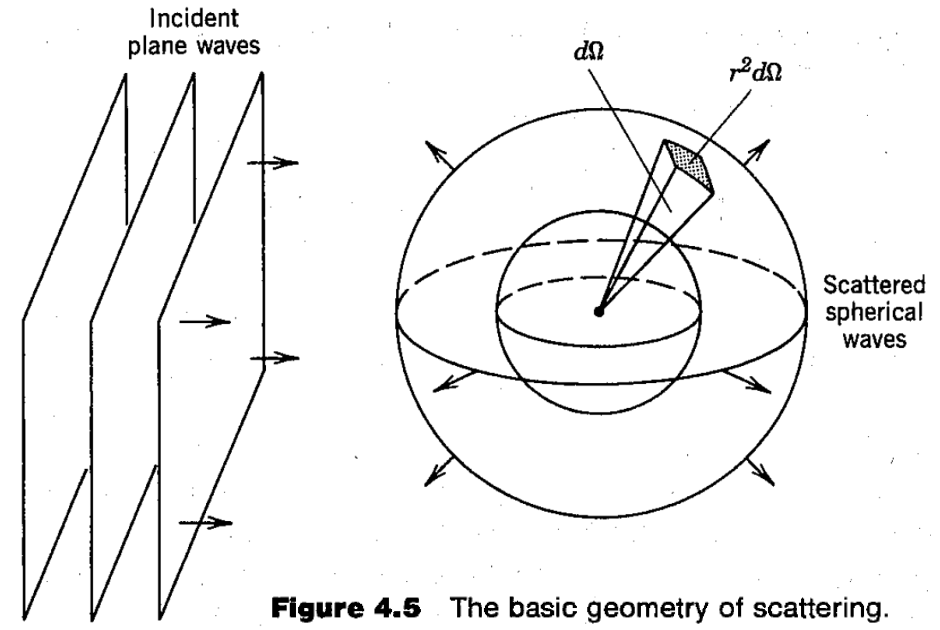
\includegraphics[width=4in]{images/scattering/scattering-geometry.png}
\caption{Geometry of Scattered Spherical Waves} \label{scattering-geometry} 
\end{figure}






In the next section we would actually solve $\psi(x)$ as an eigenstate problem using Methods of Partial Wave. 






\topic{Method of Partial Waves} 
To find $f(\theta)$, we solve the Schrodinger Equation for wave function $\psi(\uline{r}, t) = \psi(\uline{r}) e^{-iEt/\hbar}$:
\eqn{\left[ - \frac{\hbar^2}{2 \mu} \uline{\gradient}^2 + V(\uline{r}) \right] \psi (\uline{r}) = E \psi(\uline{r}) }
We've already solved for this problem for the bound state condition ($E <0$), whereas now we consider the scattering case $E>0$, with the boundary condition:
\eqn{\psi(r) \xrightarrow{r \gg r_0} \psi_{\mathrm{inc}} + \psi_{\mathrm{sc}} = e^{i \uline{k r}} + f(\theta) \frac{e^{ikr}}{r} \label{BC}}

\begin{enumerate}
\item Set-up Partial Wave: we expand the $\psi(r)$ into $\psi(r, \theta)$, notice there is no $\phi$ dependence because of $V(r)$. Then we can write $\psi(r,\theta)$ into the summation of partial waves, in which $P_l (\cos \theta)$ is the Legende Polynomial, 
\eqn{\psi(r,\theta) = \Sum_{l=0}^{\infty} R_l(r) P_l (\cos \theta) }
More rigorously we take into account $l$, 
\eqn{\psi(r,\theta) = \Sum_{l=0}^{\infty} R_l(r) i^l (2l+1) P_l (\cos \theta) }
where $P_l (\cos \theta) = Y_l^{m=0} (\theta, \phi)$. 

\item Simplify Schrodinger Equation, consider radial function: 
\begin{align}
\left. \begin{array}{c}
\left(- \frac{\hbar^2}{2 \mu} \uline{\gradient}^2 + V(\uline{r}) - E  \right) \psi(r,\theta) = 0 \\
u_l (r) = r R_l (r) 
\end{array} \right\} 
\left( -\frac{\hbar^2}{2 \mu} \pprn2 +\frac{\hbar^2 l(l+1)}{2 \mu r^2} + V(\uline{r}) - E  \right) u_l (r) &= 0 \\
\left( \pprn2 - \frac{l(l+1)}{r^2} - \frac{2\mu}{\hbar^2} V(\uline{r}) + \overbrace{\frac{2\mu}{\hbar^2} E}^{\to k^2}  \right) u_l (r) &= 0 
\end{align}

\item For $r\le r_0$, $V(r) \neq 0$: we don't actually pursue this case. Indeed, we only consider the extreme case $V (r) =0$. 
\begin{align}
\left( \pprn2 - \frac{l(l+1)}{r^2} - \frac{2\mu}{\hbar^2} V(\uline{r}) + k^2  \right) u_l (r) &= 0 
\end{align}

\item For $r>r_0$, $V(r) =0$: 
\eqn{ \left( \pprn2 - \frac{l(l+1)}{r^2} + k^2  \right) u_l (r) &= 0  }
The solution is in the form of $j_l (kr)$ (Spherical Bessel Functions) and $n_l (kr)$ (Spherical Neumann Functions):
\eqn{ \Rightarrow u_l (r) &= B_l r j_l (kr) + C_l r n_l (kr) }

\item For the extreme case $r \gg r_0, kr \gg 1$, 
\eqn{ j_l (x) &\xrightarrow{x \gg 1} \frac{1}{x} \sin \left( x - \frac{l \pi}{2} \right) & n_l (x) &\xrightarrow{x \gg 1} - \frac{1}{x} \cos \left( x - \frac{l \pi}{2} \right)  }
That is, 
\eqn{ u_l (r) \xrightarrow{kr \gg 1} \frac{B_l}{k} \sin \left( kr - \frac{l \pi}{2} \right) - \frac{C_l}{k} \cos \left( kr - \frac{l \pi}{2} \right)  = \frac{A_l}{k} \sin \left( kr - \frac{l \pi}{2} + \delta_l \right) \label{delta_l}}
in which $ \delta_l = \mbox{phase shift of each partial wave after interact with $V(r)$}.$ Thus the solution to the Schrodinger Equation for the extreme of $kr \gg 1$ is,
\eqn{ \psi(r,\theta) \xrightarrow{kr \gg 1} \Sum_{l=0}^{\infty} \frac{A_l}{kr} \sin \left( kr - \frac{l \pi}{2} + \delta_l \right) P_l (\cos \theta) \label{sol}  }
We can apply the Boundary Condition in Eq.~\ref{BC}. To do so, we need to expand 
\eqn{ f(\theta) = \Sum_{l=0}^{\infty} i^l (2l+1) f_l P_l (\cos \theta) }
and expand, 
\begin{align}
e^{ikz} &= e^{ikr \cos \theta} = \Sum_l i^l (2l+1) j_l (kr) P_l (\cos \theta) \\
& \xrightarrow{kr \gg 1} \Sum_l  \frac{i^l (2l+1)}{kr} \sin \left( kr - \frac{l \pi}{2} \right) P_l (\cos \theta) \\
&= \Sum_l  \frac{i^l (2l+1)}{kr} \frac{1}{2i} \left[ e^{ i \left( kr - \frac{l \pi}{2} \right)} - e^{ -i \left( kr - \frac{l \pi}{2} \right)} \right] P_l (\cos \theta)
\end{align}
Then we equate the coefficient before the same $l$ state (taking into account the incoming plane wave), we have the equation, 
\eqn{ a_l \sin \left( kr - \frac{l\pi}{2} + \delta_l \right) - \sin \left( kr - \frac{l \pi}{2} \right) = f_l e^{ikr} }
To simplify and solve for $f_l$, we know $f_l$ is not a function of $r$, so 
\eqn{ a_l \frac{e^{ikr - i l \pi/2 + i \delta_l } - e^{-ikr + i l\pi/2 - i \delta_l}}{2i} - \frac{e^{ikr - i l \pi/2} - e^{-ikr + i l\pi/2}}{2i} = f_l e^{ikr} }
Thus we should get, 
\eqn{ a_l &= e^{i\delta_l} & f_l &= e^{- \frac{i l \pi}{2} } \frac{e^{2i\delta_l} - 1}{2i} = (-i)^l e^{i \delta_l} \sin \delta_l }
Then we can solve for the differential cross section and the total cross section,
\begin{align}
f(\theta) &= \frac{1}{k} \Sum_{l=0}^{\infty} (2l+1) e^{i \delta_l} \sin \delta_l P_l (\cos \theta) \label{f-theta} \\
\sigma (\theta) &= |f(\theta)|^2 = \frac{1}{k^2} \left| \Sum_{l=0}^{\infty} (2l+1) e^{i \delta_l} \sin \delta_l P_l (\cos \theta) \right|^2 \label{sigma-theta} \\
\sigma &=  \int  \sigma(\theta) \dOmega = 2 \pi \int_{\pi}^0 \derivative \cos \theta |f(\theta)|^2   = \boxed{\frac{4 \pi}{k^2} \Sum_{l=0}^{\infty} (2l+1) \sin^2 \delta_l  \label{sigma} }
\end{align}
where we use the mathematically expression that 
\eqn{ \int_{\pi}^0 \derivative \cos \theta P_l (\cos \theta) P_{l'} (\cos \theta) = \frac{2 \delta_{ll'}}{2l+1} }
Notice, Eq.~\ref{f-theta} $\sim$ Eq.~\ref{sigma} are the general expression. 
\end{enumerate}

\end{document}
